\documentclass[12pt,xcolor=dvipsnames]{article}
\usepackage[utf8]{inputenc}
\usepackage[vietnamese]{babel}
\usepackage{amstext,latexsym,amsbsy,amssymb,amsmath,amsthm,amsfonts,exscale,eucal}
\usepackage{appendix}
\usepackage{algorithm}
\usepackage{graphicx}
\usepackage{xcolor}
\usepackage{hyperref}
\usepackage{indentfirst}
\usepackage{enumitem}
\usepackage{diagbox}
\usepackage{booktabs}

\usepackage[left=2.00cm, right=2.00cm, top=2.00cm, bottom=2.00cm]{geometry}
\setlength{\parskip}{5pt}%khoảng cách dòng
\renewcommand{\baselinestretch}{1.15}
\theoremstyle{definition}
\newtheorem{vd}{Ví dụ}[section]
\newtheorem*{giai}{Giải}
\newtheorem{bt}{Bài tập}
\renewcommand{\l}{\left}
\renewcommand{\r}{\right}
\date{}

\begin{document}
\begin{bt}
(Mô hình giá quyền chọn cổ phiếu). Mô hình giá của cổ phiếu tại ngày $T$ theo cách chọn châu Âu (European Call Option) được miêu tả theo mô hình Black-Scholes:
\[
S^{(T)} = S^{(0)} \exp\left\{\left(r - \frac{\sigma^2}{2}\right)\frac{T}{365} + \sigma Z \sqrt{\frac{T}{365}}\right\},
\]
với $Z \sim \mathcal{N}(0,1)$. Giá hợp lý của quyền chọn mua:
\[
C = \exp\left(-\frac{rT}{365}\right) \max\left\{0, S^{(T)} - K\right\}.
\]
\begin{enumerate}
    \item[(a)] Xét $S^{(0)}=50$, $K=52$, $\sigma=0.5$, $r=0.05$, $T=30$. Xác định giá hợp lý phải trả. So sánh với $2.10$.
    \item[(b)] Mô hình Asian Call Option: $S^{(t+1)} = S^{(t)}\exp\left\{\frac{r-\sigma^2/2}{365} + \frac{\sigma Z^{(t)}}{\sqrt{365}}\right\}$. Xác định ước lượng $\mathbb{E}(A)$.
\end{enumerate}
\end{bt}

\begin{giai}
\textbf{1. European Call Option (Quyền chọn mua kiểu châu Âu)}

Ước tính Monte Carlo với $n = 100{,}000$ mô phỏng. Với mỗi lần mô phỏng $i$, ta sinh $Z_i \sim \mathcal{N}(0,1)$, tính:
\[
S_i^{(T)} = 50 \cdot \exp\left\{\left(0.05 - \frac{0.25}{2}\right)\frac{30}{365} + 0.5 \cdot Z_i \cdot \sqrt{\frac{30}{365}}\right\},
\]
\[
C_i = \exp\left(-\frac{0.05 \times 30}{365}\right) \max\left\{0,\ S_i^{(T)} - 52\right\}.
\]
Ước lượng giá hợp lý: $\bar{C} = \frac{1}{n}\sum_{i=1}^{n} C_i$.

\textit{Kết quả:}
\begin{itemize}
    \item Ước lượng Monte Carlo: $\bar{C} = 2.0988$
    \item Sai số chuẩn (SE): $0.0125$
    \item Khoảng tin cậy 95\%: $[2.0743,\ 2.1233]$
    \item Giá trị lý thuyết: $2.10$
    \item Sai số tuyệt đối: $|2.0988 - 2.10| = 0.0012$
\end{itemize}

\textit{Nhận xét:} Giá trị ước lượng Monte Carlo ($2.0988$) rất gần với giá trị lý thuyết ($2.10$), và giá trị lý thuyết nằm trong khoảng tin cậy 95\%. Điều này xác nhận tính chính xác của phương pháp Monte Carlo.

\begin{center}
    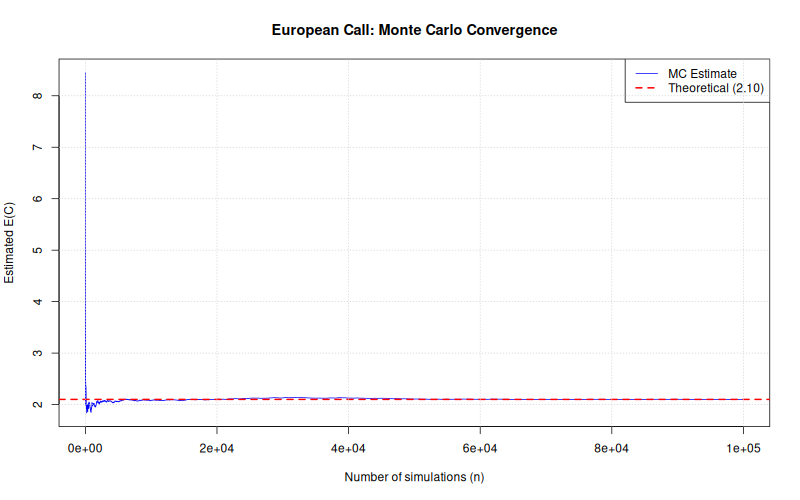
\includegraphics[width=0.8\textwidth]{european_convergence.png}
\end{center}

Hình trên cho thấy ước lượng Monte Carlo hội tụ nhanh về giá trị lý thuyết $2.10$ (đường đỏ nét đứt) khi số lần mô phỏng tăng.

\textbf{2. Asian Call Option (Quyền chọn mua kiểu châu Á)}

Với mỗi mô phỏng $i$, ta tạo đường đi giá cổ phiếu theo từng ngày:
\[
S^{(t+1)} = S^{(t)} \exp\left\{\frac{r - \sigma^2/2}{365} + \frac{\sigma Z^{(t)}}{\sqrt{365}}\right\}, \quad t = 0, 1, \ldots, T-1,
\]
với $Z^{(t)} \sim \mathcal{N}(0,1)$ độc lập. Giá trị quyền chọn:
\[
A_i = \exp\left(-\frac{rT}{365}\right) \max\left\{0,\ \bar{S}_i - K\right\}, \quad \text{với } \bar{S}_i = \frac{1}{T}\sum_{t=1}^{T} S_i^{(t)}.
\]

\textit{Kết quả:}
\begin{itemize}
    \item Ước lượng Monte Carlo: $\bar{A} = 0.9535$
    \item Sai số chuẩn (SE): $0.0064$
    \item Khoảng tin cậy 95\%: $[0.9411,\ 0.9660]$
\end{itemize}

\textbf{3. So sánh European và Asian Call Option}

\begin{table}[h]
\centering
\begin{tabular}{lcc}
\toprule
\textbf{Loại quyền chọn} & \textbf{Giá ước lượng} & \textbf{Sai số chuẩn} \\
\midrule
European Call & 2.0988 & 0.0125 \\
Asian Call    & 0.9535 & 0.0064 \\
\bottomrule
\end{tabular}
\caption{So sánh giá quyền chọn European và Asian}
\end{table}

\textit{Giải thích:} Giá quyền chọn Asian ($0.9535$) thấp hơn đáng kể so với European ($2.0988$). Nguyên nhân:
\begin{itemize}
    \item Quyền chọn Asian dựa trên \textbf{giá trung bình} $\bar{S}$ thay vì giá tại thời điểm cuối $S^{(T)}$.
    \item Theo bất đẳng thức Jensen và tính chất của trung bình, phương sai của $\bar{S}$ nhỏ hơn phương sai của $S^{(T)}$: việc lấy trung bình có tác dụng \textit{làm mượt} (smoothing), giảm độ biến động hiệu dụng.
    \item Khi độ biến động giảm, xác suất $\bar{S}$ vượt qua giá thực hiện $K = 52$ cũng giảm, dẫn đến payoff trung bình thấp hơn.
    \item Quyền chọn Asian thường được sử dụng trong thực tế để giảm rủi ro thao túng giá tại thời điểm đáo hạn.
\end{itemize}

\begin{center}
    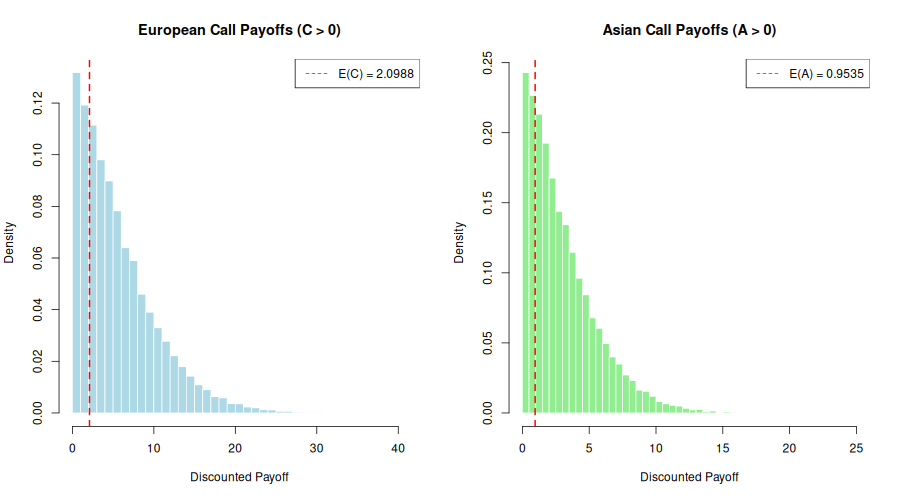
\includegraphics[width=0.9\textwidth]{option_comparison.png}
\end{center}

\textbf{Mã nguồn:} File \texttt{exercise\_04.R} chứa toàn bộ code thực hiện mô phỏng.
\end{giai}
\end{document}
